\documentclass{article}
    \usepackage[a4paper,top=3cm,bottom=3cm,left=2.5cm,right=2.5cm,marginparwidth=1.75cm]{geometry}
    \title{Piano di Progetto}
    \usepackage[T1]{fontenc}
    %\usepackage{lmodern}
    \usepackage[utf8]{inputenc}
    \usepackage[italian]{babel}
    \usepackage{amsmath}
    \usepackage{booktabs}
    \usepackage{longtable}
    \usepackage{wrapfig}
    \usepackage{mdframed}
    \usepackage{hyperref}
    \usepackage{adjustbox}
    \usepackage{lastpage}
    
    %% HEADER
    \usepackage[sfdefault,lf]{carlito}
    %% The 'lf' option for lining figures
    %% The 'sfdefault' option to make the base font sans serif
    \usepackage[parfill]{parskip}
    \renewcommand*\oldstylenums[1]{\carlitoOsF #1}
    \usepackage{fancyhdr}
    %\usepackage{natbib}
    %\usepackage{authblk}
    \setlength{\headheight}{41pt}
    
    \fancyhead[L]{WatchDoge: Documento di Specifica dei Requisiti}
    \fancyhead[R]{
    
\includegraphics[width=4cm]{gfx/logo.pdf}
    }
    \fancyfoot[C]{\sffamily\fontsize{9pt}{9pt}\selectfont{\thepage/\pageref{LastPage}}}
    \pagestyle{fancy}
    
    \makeatletter
    
    \newcommand{\spacedlowsmallcaps}[1]{\textbf{#1}}
    \newcommand{\titleColor}{}
    \makeatother
    
    \usepackage{graphicx}
    \usepackage[absolute]{textpos}
    \usepackage[table]{xcolor}
    \definecolor{lightgray}{gray}{0.9}
    
    \begin{document}
    \rowcolors{1}{}{lightgray}
    \thispagestyle{empty}
    \setlength{\TPHorizModule}{1mm}
    \setlength{\TPVertModule}{1mm}
    
    \begingroup
    \fontsize{11pt}{11pt}\selectfont
    \linespread{1.05}
    
    \begin{textblock}{50}(0,0)
    \noindent 
\includegraphics{gfx/00_cafoscari}
    \noindent \end{textblock}
    ~
    \begin{textblock}{143}(47,42)
    
    \noindent {\LARGE{}Progetto per\\Ingegneria del Software \emph{(CT0090)}}\\
    \vspace{30pt}
    
    %\vspace{30pt}
    
    
    \noindent %
    \begin{minipage}[t]{1\columnwidth}%
    \leavevmode
    \titleColor
    \raggedright
    \Huge
    
\includegraphics[width=12cm]{gfx/logo.pdf}
    \vspace{10pt}
    
    WatchDoge:
    Documento di Specifica dei Requisiti \\
    \LARGE{Versione 1.0 - 2 novembre 2018}
    \end{minipage}
    
    \vspace{150pt}
    
    
    \noindent {\large{}\spacedlowsmallcaps{{\large{}Redazione}}}{\large \par}
    \begin{itemize}
    \item   Dario Lazzaro
    \item   Giovanni Scodeller
    \item   Giulio Zausa
    \item   Samuele Casarin
    \item   Sandro Baccega
    \end{itemize}
    
    \vspace{20pt}
    
    
    \noindent {\large{}\spacedlowsmallcaps{{\large{}Approvazione}}}{\large \par}
    \begin{itemize}
    \item   Dario Lazzaro
    \item   Samuele Casarin
    \item   Sandro Baccega
    \end{itemize}
    \end{textblock}
    \endgroup
    \pagebreak
    
    %
    %	inizio roba vera e propria
    %
    
    \tableofcontents
    
    \pagebreak
      
    \section{Introduzione}
    
    \subsection{Scopo del documento}
    
    Il documento ha lo scopo di descrivere in modo dettagliato:
    \begin{itemize}
    \item il funzionamento del sistema che andremo a realizzare;
    \item le modalità d’uso;
    \item il modo in cui l’utente può interagire con il sistema.
    \end{itemize}
    
    Valuteremo, inoltre, i requisiti funzionali e non funzionali che il sistema dovrà rispettare, procedendo con:
    \begin{itemize}
    \item lo studio di fattibilità (interno al gruppo);
    \item l’analisi dei requisiti e la loro definizione;
    \item fornire la specifica dei requisiti;
    \item la convalida e la verifica del tutto.
    \end{itemize}
    
    \vspace{10pt}
    \begin{figure}[htbp]
    \centering
    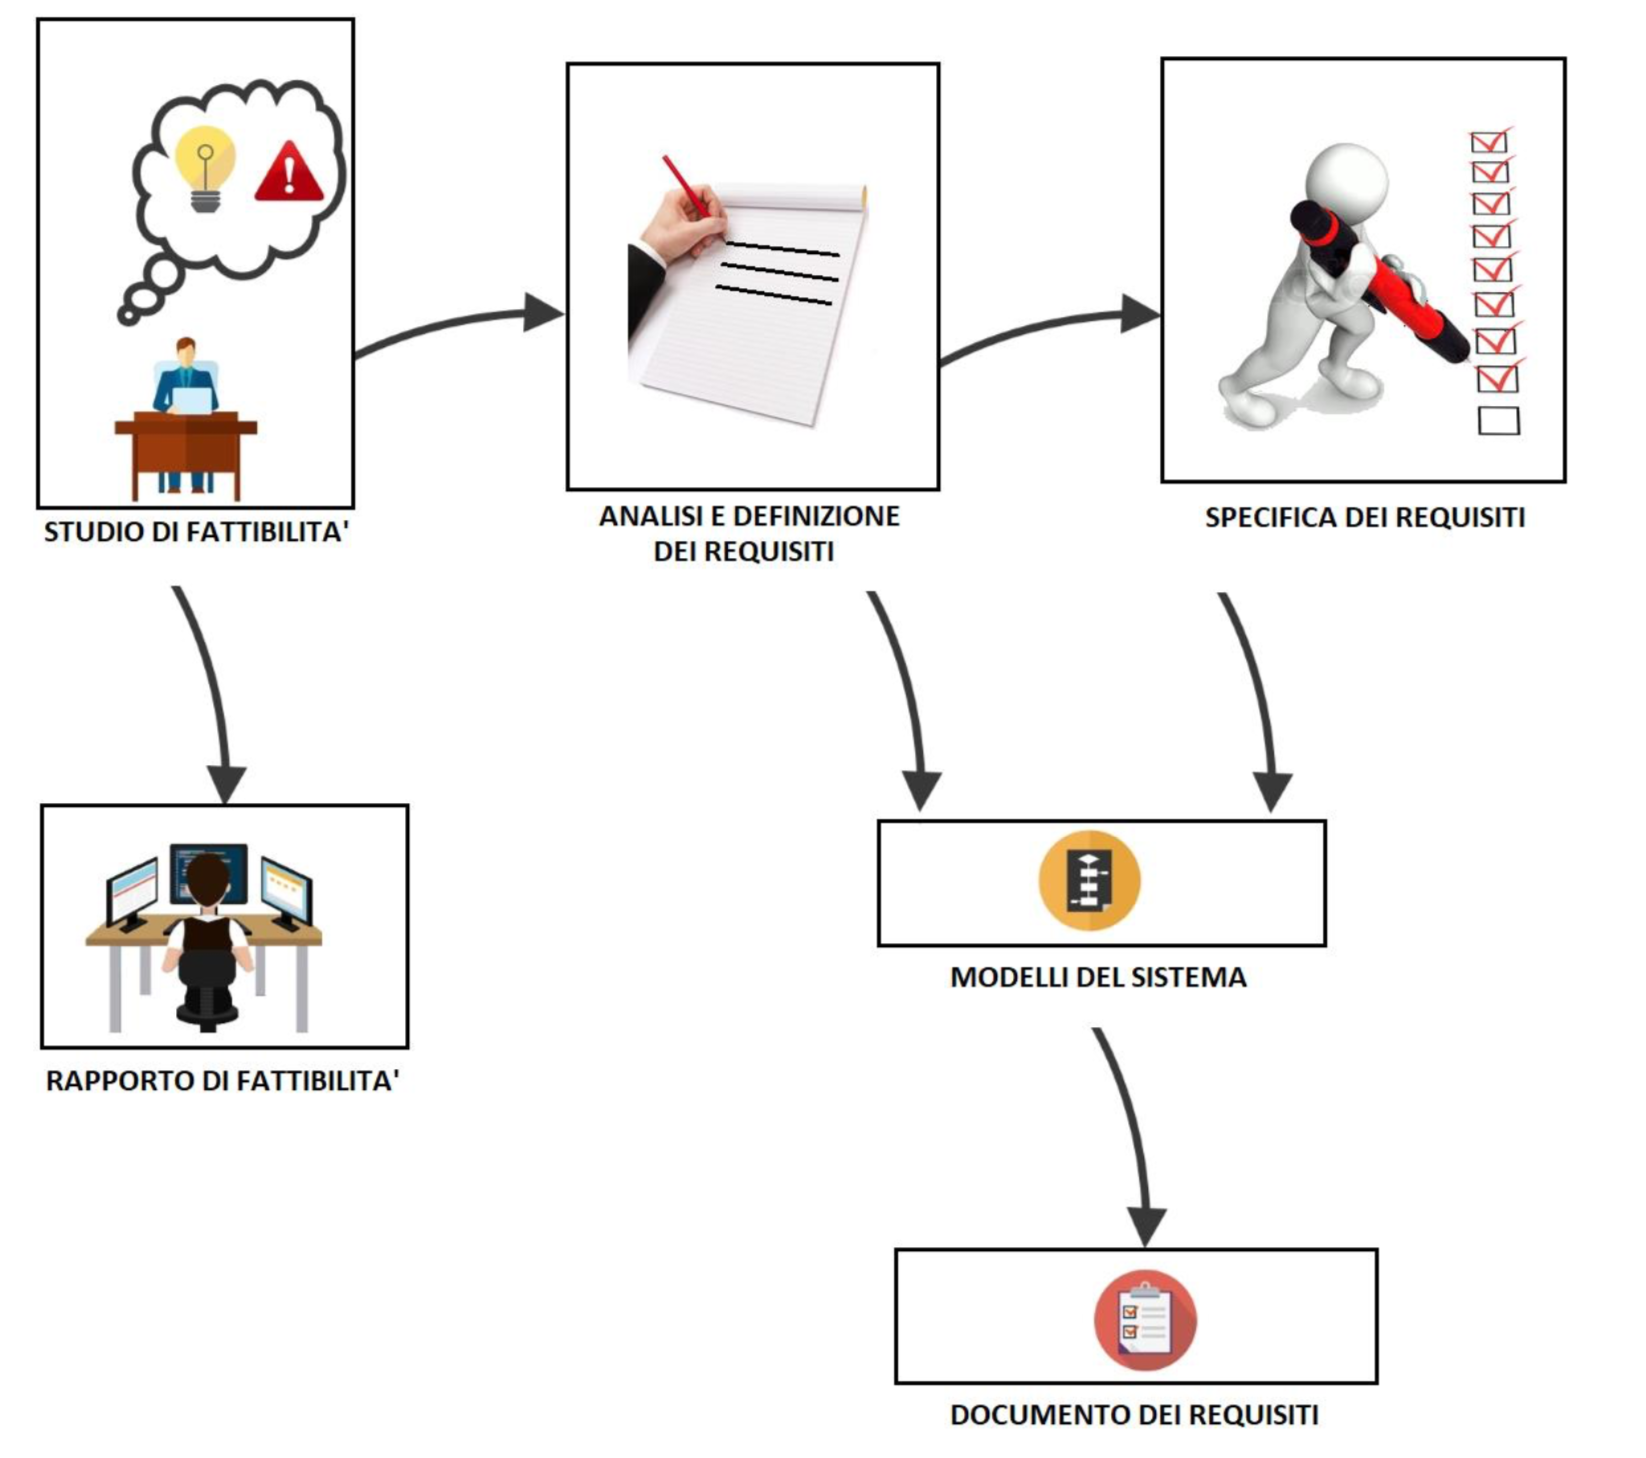
\includegraphics[width=12cm]{cazzate.png}
    \end{figure}
    
    \subsection{Descrizione del documento}
    
    Il documento è organizzato in otto paragrafi che trattano i seguenti argomenti:
    
    \begin{enumerate}
    \item \textbf{Introduzione:} descrizione iniziale del documento e dei suoi sottopunti.
    \item \textbf{Glossario:} è un elenco dettagliato dei termini di uso tecnico utilizzati nel documento.
    \item \textbf{Modelli di sistema:} mostra la descrizione della struttura vera e propria dell’app Android e il Doge attraverso l’utilizzo degli use case del linguaggio UML2.
    \item \textbf{Definizione dei requisiti funzionali:} descrizione dei servizi che il sistema dovrà necessariamente fornire, nel momento in cui l’applicazione verrà rilasciata.
    \item \textbf{Definizione dei requisiti non funzionali:} descrizione dei vincoli del sistema e del processo di sviluppo.
    \item \textbf{Evoluzione del sistema:} i servizi e le modifiche che potranno essere apportate al sistema (applicazione e doge) in futuro.
    \item \textbf{Specifica dei requisiti:} spiegazione nel dettaglio dei requisiti funzionali.
    \end{enumerate}
    
    \subsection{Funzionalità di progetto}
    
    L'obiettivo del progetto è lo sviluppo di un sistema anti intrusione destinato all'uso domestico.
    Tale sistema sarà composto principalmente da due sottosistemi:
    \begin{itemize}
    \item un \textbf{dispositivo} \textit{(Doge)} connesso ad Internet che, quando abilitato, rileva le intrusioni all'interno dell'ambiente domestico (entro certi limiti), notificando l'utente tramite l'applicazione Android;
    \item un'\textbf{applicazione Android} (WatchDoge) che abilita/disabilita Doge su decisione dell'utente e notifica l'utente riguardo le segnalazioni ricevute da Doge.
    \end{itemize}
    
    Questo sistema andrà a realizzare una componente specifica dei sistemi \textit{Smart Home}, ovvero la rilevazione di intrusioni, permettendo però di avere delle funzionalità aggiuntive, come la configurabilità e la possibilità di tenere traccia dello storico degli avvenimenti.
    
    \section{Glossario}
    
    \begin{figure}[htbp]
    \centering
    \begin{tabular}{l p{12cm}}
    \textbf{WatchDoge} & Il nome scelto per l'applicazione Android. \\
    \textbf{Doge} & Il nome scelto per il dispositivo. \\
    \textbf{Android} & Sistema operativo per dispositivi mobili sviluppato da Google Inc. e basato sul kernel Linux. \\
    \textbf{Accoppiamento} & L'azione di associazione di uno smartphone con un dispositivo (Doge). \\
    \textbf{EV3} & Hardware realizzato da Lego composto da una unità centrale (su cui gira il kernel Linux) e sensori di rilevazione. \\
    \textbf{Smart Home} & Categoria di apparecchi atti ad automatizzare processi di gestione della casa, mediante nuove tecnologie ed internet. \\
    \textbf{Anti intrusione} & Sistema atto a rilevare e prevenire accessi non autorizzati in determinati spazi. \\
    \end{tabular}
    \end{figure}
    
    \section{Modelli del Sistema}
    
    In questa sezione verranno elencati i casi d’uso del sistema.
    Attraverso l’analisi di ognuno di essi, che si compone di una breve descrizione (Tabella 1) e di un diagramma \textit{UML}, si vogliono mostrare i diversi scenari in cui un determinato attore interagisce con il sistema.
    
    \begin{figure}[htbp]
    \centering
    \begin{tabular}{|c|l|}
    \hline
    \textbf{Codice} & \textit{Codice univoco del caso d'uso} \\ \hline
    \textbf{Nome} & \textit{Nome del caso d'uso} \\ \hline
    \textbf{Scopo} & \textit{Descrive il problema che il caso d'uso si pone di risolvere} \\ \hline
    \textbf{Attori} & \textit{I soggetti (non necessariamente persone) coinvolti nel caso d'uso} \\ \hline
    \textbf{Precondizioni} & \textit{Indica quali requisiti devono essere soddisfatti all'istante dell'applicazione del caso d'uso} \\ \hline
    \textbf{Trigger} & \textit{Indica quale evento deve verificarsi per l'applicazione del caso d'uso} \\ \hline
    \textbf{Descrizione} & \textit{Spiegazione ad alto livello del modo in cui il caso d'uso raggiunge il suo scopo} \\ \hline
    \textbf{Alternative} & \textit{Insieme di casi d'uso che permettono di raggiungere lo stesso scopo} \\ \hline
    \textbf{Postcondizioni} & \textit{Indica le conseguenze dell'applicazione del caso d'uso} \\ \hline
    \end{tabular}
    \caption{Template di base per la descrizione dei casi d’uso}
    \end{figure}
    
    \begin{figure}[htbp]
    \begin{adjustbox}{center}
    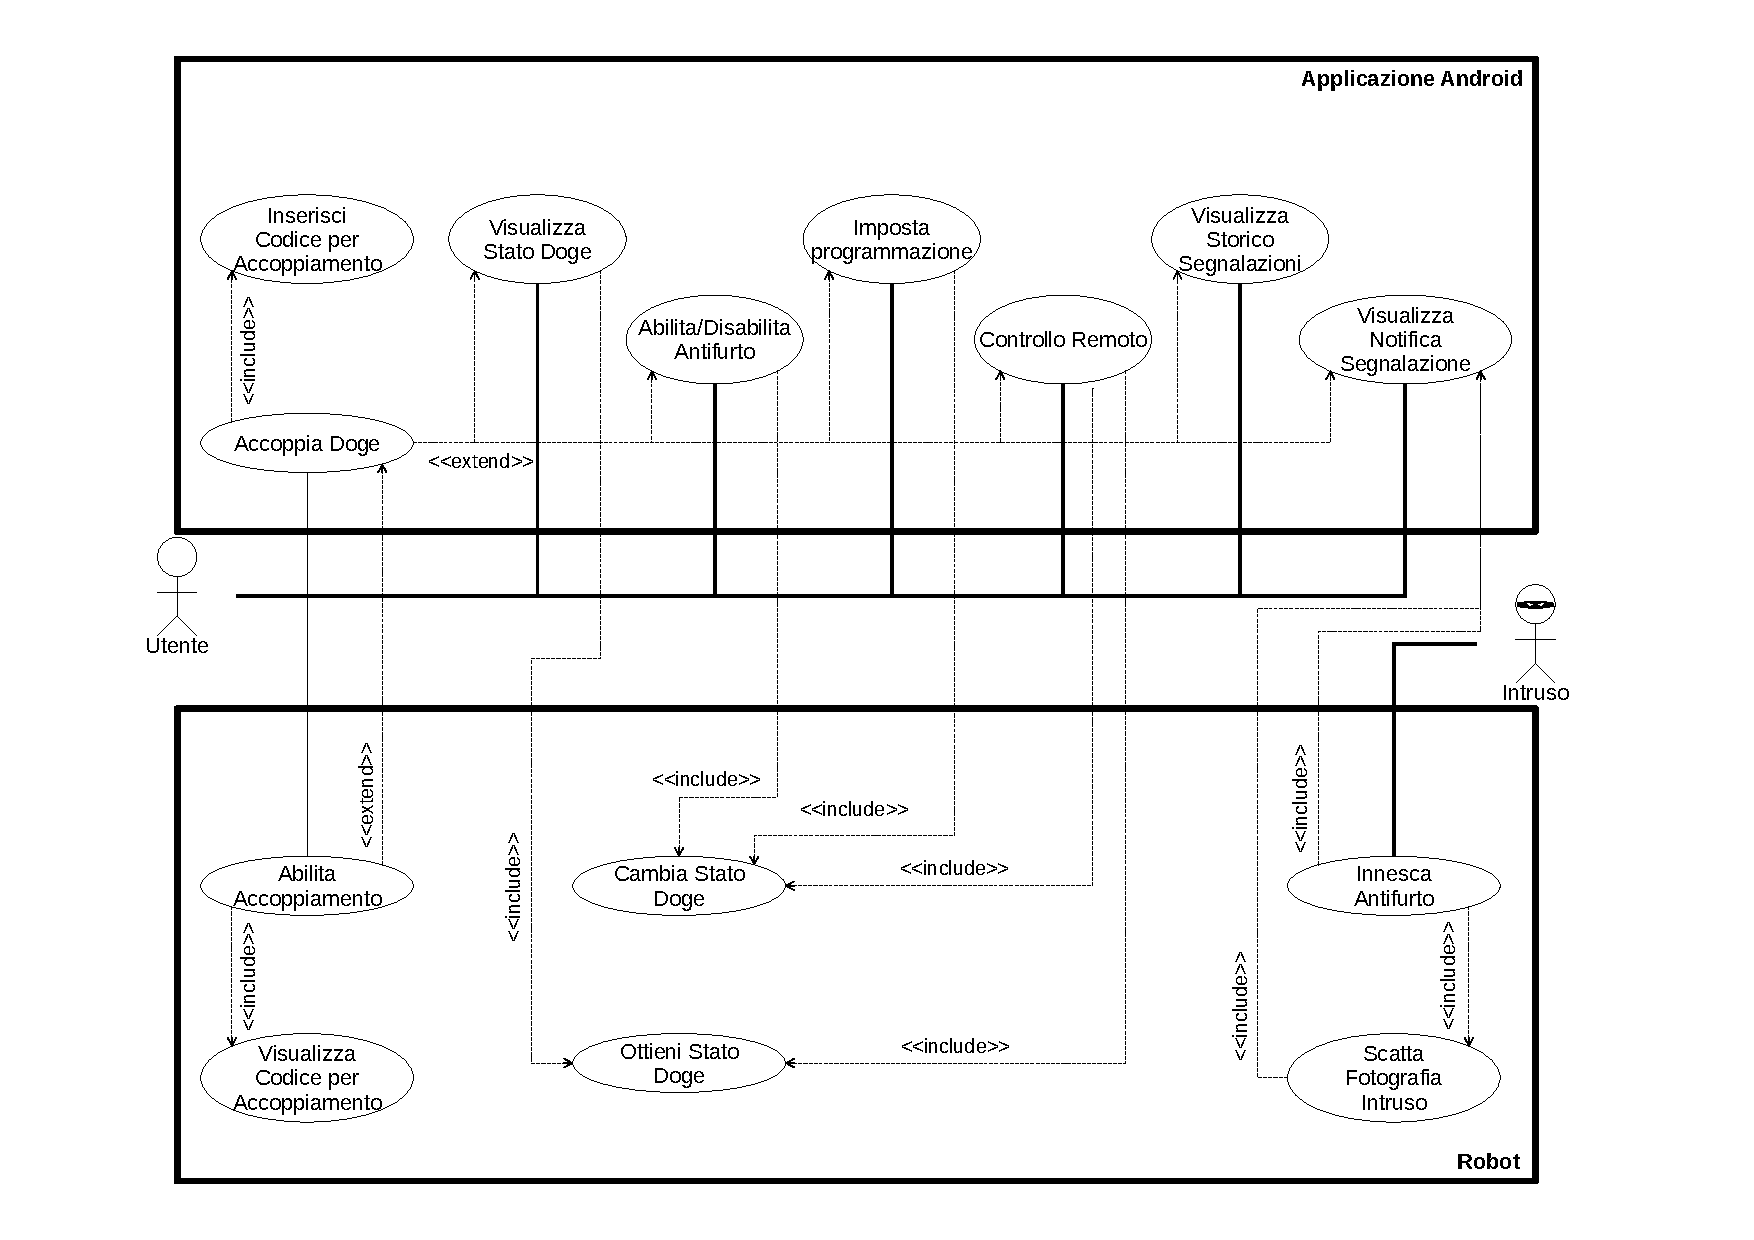
\includegraphics[width=20cm]{UC-Diagram.pdf}
    \end{adjustbox}
    \caption{Diagramma UML dei vari casi d'uso}
    \end{figure}
    
    \pagebreak
    
    \begin{adjustbox}{center}
    \begin{tabular}{|c|p{10cm}|}
    \hline
    \textbf{Codice} & UC-01 \\
    \textbf{Nome} & Abilita Accoppiamento \\
    \textbf{Scopo} & Associare il Doge ad un dispositivo Android per permetterne il controllo all'utente. \\
    \textbf{Attori} & Utente \\
    \textbf{Precondizioni} & - \\
    \textbf{Trigger} & Pressione del pulsante \emph{Abilita accoppiamento} (Doge) \\
    \textbf{Descrizione} & Il Doge accetta richieste di accoppiamento per un certo tempo. \\
    \textbf{Alternative} & - \\
    \textbf{Postcondizioni} & Il Doge è accoppiato con un dispositivo Android, oppure non è accoppiato \\
    \hline
    \end{tabular}
    \end{adjustbox}
    
    \begin{adjustbox}{center}
    \begin{tabular}{|c|p{10cm}|}
    \hline
    \textbf{Codice} & UC-02 \\
    \textbf{Nome} & Visualizza Codice per Accoppiamento \\
    \textbf{Scopo} & Mitigare la presa di controllo indesiderata del Doge da parte di qualcun altro diverso dall'utente. \\
    \textbf{Attori} & Utente \\
    \textbf{Precondizioni} & UC-01 \\
    \textbf{Trigger} & Il Doge riceve una richiesta di accoppiamento. \\
    \textbf{Descrizione} & Il Doge visualizza un codice con cui il dispositivo che ha inviato la richiesta di accoppiamento deve rispondere per poter completare la
    procedura di accoppiamento. \\
    \textbf{Alternative} & - \\
    \textbf{Postcondizioni} & Il successo della verifica garantisce che il dispositivo che ha inviato la richiesta di accoppiamento è effettivamente quello dell'utente. \\
    \hline
    \end{tabular}
    \end{adjustbox}
    
    \begin{adjustbox}{center}
    \begin{tabular}{|c|p{10cm}|}
    \hline
    \textbf{Codice} & UC-03 \\
    \textbf{Nome} & Accoppia Doge \\
    \textbf{Scopo} & Associare il dispositivo Android al Doge per permetterne il controllo all'utente. \\
    \textbf{Attori} & Utente \\
    \textbf{Precondizioni} & Connessione alla stessa rete del Doge, UC-01 \\
    \textbf{Trigger} & Primo avvio dell'applicazione Android e pressione del pulsante \emph{Accoppia Doge} (applicazione Android) \\
    \textbf{Descrizione} & L'applicazione Android cerca Doge presenti nella stessa rete dello smartphone entro un certo tempo. Al termine, l'applicazione Android
    visualizza la lista di Doge trovati, permettendo all'utente di
    selezionare quello da associare. \\
    \textbf{Alternative} & - \\
    \textbf{Postcondizioni} & Il dispositivo Android è accoppiato con il Doge \\
    \hline
    \end{tabular}
    \end{adjustbox}
    
    \begin{adjustbox}{center}
    \begin{tabular}{|c|p{10cm}|}
    \hline
    \textbf{Codice} & UC-04 \\
    \textbf{Nome} & Inserisci Codice per Accoppiamento \\
    \textbf{Scopo} & Mitigare la presa di controllo indesiderata del Doge da parte di qualcun altro diverso dall'utente. \\
    \textbf{Attori} & Utente \\
    \textbf{Precondizioni} & UC-03 \\
    \textbf{Trigger} & Selezione di un Doge da associare \\
    \textbf{Descrizione} & L'utente inserisce il codice di accoppiamento visualizzato dal Doge e lo inserisce in un apposito campo. Successivamente, l'applicazione
    Android invia il codice al Doge per la verifica. \\
    \textbf{Alternative} & - \\
    \textbf{Postcondizioni} & Il successo della verifica garantisce che il dispositivo che ha inviato la richiesta di accoppiamento al Doge è effettivamente quello
    dell'utente. \\
    \hline
    \end{tabular}
    \end{adjustbox}
    
    \begin{adjustbox}{center}
    \begin{tabular}{|c|p{10cm}|}
    \hline
    \textbf{Codice} & UC-05 \\
    \textbf{Nome} & Visualizza Stato Doge \\
    \textbf{Scopo} & Consentire all'utente di visualizzare in tempo reale le informazioni relative al Doge. \\
    \textbf{Attori} & Utente \\
    \textbf{Precondizioni} & UC-03 \\
    \textbf{Trigger} & Aprire l'applicazione Android \\
    \textbf{Descrizione} & L'utente visualizza in tempo reale se l'antifurto è abilitato oppure no e la sua programmazione attraverso un'apposita interfaccia
    grafica. \\
    \textbf{Alternative} & - \\
    \textbf{Postcondizioni} & L'utente è al corrente dello stato del Doge. \\
    \hline
    \end{tabular}
    \end{adjustbox}
    
    \begin{adjustbox}{center}
    \begin{tabular}{|c|p{10cm}|}
    \hline
    \textbf{Codice} & UC-06 \\
    \textbf{Nome} & Abilita/Disabita Doge \\
    \textbf{Scopo} & Consentire all'utente di attivare/disattivare la funzione di antifurto del Doge. \\
    \textbf{Attori} & Utente \\
    \textbf{Precondizioni} & UC-03 \\
    \textbf{Trigger} & Pressione del pulsante \emph{ON/OFF} (applicazione Android) \\
    \textbf{Descrizione} & L'utente cambia lo stato del Doge ad attivo/disattivo. \\
    \textbf{Alternative} & - \\
    \textbf{Postcondizioni} & Il Doge è attivo/disattivo. \\
    \hline
    \end{tabular}
    \end{adjustbox}
    
    \begin{adjustbox}{center}
    \begin{tabular}{|c|p{10cm}|}
    \hline
    \textbf{Codice} & UC-07 \\
    \textbf{Nome} & Imposta Programmazione \\
    \textbf{Scopo} & Consentire all'utente di decidere quando il Doge deve attivarsi/disattivarsi automaticamente in determinate fasce
    orarie. \\
    \textbf{Attori} & Utente \\
    \textbf{Precondizioni} & UC-03 \\
    \textbf{Trigger} & Pressione del pulsante \emph{Programma} \\
    \textbf{Descrizione} & L'utente abilita/disabilita la modalità automatica attraverso un interrutore e imposta le fasce orarie di attivazione del Doge
    attraverso una tabella oraria settimanale. \\
    \textbf{Alternative} & - \\
    \textbf{Postcondizioni} & Il Doge è configurato in modalità automatica per attivarsi negli orari stabiliti dall'utente. \\
    \hline
    \end{tabular}
    \end{adjustbox}
    
    \begin{adjustbox}{center}
    \begin{tabular}{|c|p{10cm}|}
    \hline
    \textbf{Codice} & UC-08 \\
    \textbf{Nome} & Controllo Remoto \\
    \textbf{Scopo} & Consentire all'utente di guardare in tempo reale le immagini catturate dal Doge e spostare la visuale. \\
    \textbf{Attori} & Utente \\
    \textbf{Precondizioni} & UC-03 \\
    \textbf{Trigger} & Pressione del pulsante \emph{Controllo remoto} \\
    \textbf{Descrizione} & L'utente può connettersi da remoto al Doge e visualizza le immagini catturate dalla fotocamera incorporata; inoltre, attraverso dei pulsanti
    direzionali, può spostare la visuale della fotocamera in base all'angolo
    di rotazione. \\
    \textbf{Alternative} & - \\
    \textbf{Postcondizioni} & L'utente acquisisce una panoramica istantanea dell'ambiente dove è disposto il Doge. \\
    \hline
    \end{tabular}
    \end{adjustbox}
    
    \begin{adjustbox}{center}
    \begin{tabular}{|c|p{10cm}|}
    \hline
    \textbf{Codice} & UC-09 \\
    \textbf{Nome} & Cambia Stato Doge \\
    \textbf{Scopo} & Attivare/disattivare/configurare una o più funzioni del Doge. \\
    \textbf{Attori} & Utente \\
    \textbf{Precondizioni} & UC-03 \\
    \textbf{Trigger} & Una richiesta proveniente dall'applicazione Android \\
    \textbf{Descrizione} & Attraverso l'interfaccia grafica, l'utente invia una richiesta al Doge per cambiare il suo stato. \\
    \textbf{Alternative} & - \\
    \textbf{Postcondizioni} & Lo stato del Doge viene cambiato a seconda della richiesta inviata. \\
    \hline
    \end{tabular}
    \end{adjustbox}
    
    \begin{adjustbox}{center}
    \begin{tabular}{|c|p{10cm}|}
    \hline
    \textbf{Codice} & UC-10 \\
    \textbf{Nome} & Ottieni Stato Doge \\
    \textbf{Scopo} & Consentire all'applicazione Android di riportare le informazioni relative alle funzioni del Doge. \\
    \textbf{Attori} & Utente \\
    \textbf{Precondizioni} & UC-03 \\
    \textbf{Trigger} & Una richiesta proveniente dall'applicazione Android \\
    \textbf{Descrizione} & L'applicazione Android invia una richiesta al Doge per ottenere il suo stato. \\
    \textbf{Alternative} & - \\
    \textbf{Postcondizioni} & L'applicazione Android ottiene lo stato del Doge a seconda della richiesta inviata. \\
    \hline
    \end{tabular}
    \end{adjustbox}
    
    \begin{adjustbox}{center}
    \begin{tabular}{|c|p{10cm}|}
    \hline
    \textbf{Codice} & UC-11 \\
    \textbf{Nome} & Visualizza Storico Segnalazioni \\
    \textbf{Scopo} & Consentire all'utente di avere un archivio delle segnalazioni di intrusioni rilevate dal Doge. \\
    \textbf{Attori} & Utente \\
    \textbf{Precondizioni} & UC-03 \\
    \textbf{Trigger} & Pressione del pulsante \emph{Storico} (applicazione Android) \\
    \textbf{Descrizione} & L'applicazione Android visualizza la lista delle ultime segnalazioni. \\
    \textbf{Alternative} & - \\
    \textbf{Postcondizioni} & L'utente ha una visione generale delle segnalazioni rilevate dal Doge. \\
    \hline
    \end{tabular}
    \end{adjustbox}
    
    \begin{adjustbox}{center}
    \begin{tabular}{|c|p{10cm}|}
    \hline
    \textbf{Codice} & UC-12 \\
    \textbf{Nome} & Visualizza Notifica Segnalazione \\
    \textbf{Scopo} & Consentire all'utente di ricevere immediatamente una segnalazione di intrusione. \\
    \textbf{Attori} & Utente \\
    \textbf{Precondizioni} & UC-03 \\
    \textbf{Trigger} & Ricezione di una segnalazione dal Doge \\
    \textbf{Descrizione} & L'applicazione Android mostra una notifica con lo scopo di avvertire l'utente di un'intrusione rilevata dal Doge. Inoltre, alla notifica
    viene allegata un'immagine dell'intruso. \\
    \textbf{Alternative} & - \\
    \textbf{Postcondizioni} & L'utente può essere informato immediatamente quando viene rilevata un'intrusione. \\
    \hline
    \end{tabular}
    \end{adjustbox}
    
    \begin{adjustbox}{center}
    \begin{tabular}{|c|p{10cm}|}
    \hline
    \textbf{Codice} & UC-13 \\
    \textbf{Nome} & Innesca Antifurto \\
    \textbf{Scopo} & Mitigare le intrusioni all'interno dell'ambiente del Doge. \\
    \textbf{Attori} & Intruso \\
    \textbf{Precondizioni} & UC-03 \\
    \textbf{Trigger} & La fotocamera del Doge rileva del movimento all'interno dell'ambiente \\
    \textbf{Descrizione} & Il Doge invia una segnalazione di intrusione al dispositivo accoppiato ed emette un suono d'allarme. \\
    \textbf{Alternative} & - \\
    \textbf{Postcondizioni} & L'intruso viene rilevato e la sua presenza viene segnalata all'utente. \\
    \hline
    \end{tabular}
    \end{adjustbox}
    
    \begin{adjustbox}{center}
    \begin{tabular}{|c|p{10cm}|}
    \hline
    \textbf{Codice} & UC-14 \\
    \textbf{Nome} & Scatta Fotografia Intruso \\
    \textbf{Scopo} & Fornire all'utente un'immagine dell'intruso per tentare la sua identificazione. \\
    \textbf{Attori} & Utente \\
    \textbf{Precondizioni} & UC-13 \\
    \textbf{Trigger} & La fotocamera del Doge rileva del movimento all'interno dell'ambiente \\
    \textbf{Descrizione} & Il Doge invia un immagine dalla fotocamera puntata nella direzione in cui ha rilevato del movimento, dove probabilmente è presente
    l'intruso. \\
    \textbf{Alternative} & - \\
    \textbf{Postcondizioni} & L'utente potrebbe avere una prova per identificare l'intruso. \\
    \hline
    \end{tabular}
    \end{adjustbox}
    
    \subsection{Definizione dei Requisiti Funzionali}
    
    \subsubsection{Doge}
    
    \begin{adjustbox}{center}
    \begin{tabular}{|c|p{10cm}|}
    \hline
    \textbf{Nome} & Accoppia Doge \\
    \textbf{ID} & FR-01 \\
    \textbf{Descrizione} & Doge deve connettersi allo smartphone del proprietario. \\
    \textbf{Motivazione} & Possibilità di visualizzare informazioni e comandare l'apparato a distanza, grazie ad una connessione via rete. \\
    \textbf{Influisce} & Funzionalità principale del sistema d'antifurto. \\
    \textbf{Specifica} & FRS-01 \\
    \hline
    \end{tabular}
    \end{adjustbox}
    
    ~
    
    \begin{adjustbox}{center}
    \begin{tabular}{|c|p{10cm}|}
    \hline
    \textbf{Nome} & Rileva Intrusi \\
    \textbf{ID} & FR-02 \\
    \textbf{Descrizione} & Doge deve accorgersi di movimenti all'interno dell'ambiente. \\
    \textbf{Motivazione} & Individuare eventuali intrusi. \\
    \textbf{Influisce} & Invio di una segnalazione all'utente. \\
    \textbf{Specifica} & FRS-02 \\
    \hline
    \end{tabular}
    \end{adjustbox}
    
    ~
    
    \begin{adjustbox}{center}
    \begin{tabular}{|c|p{10cm}|}
    \hline
    \textbf{Nome} & Emette Suono d'Allarme \\
    \textbf{ID} & FR-03 \\
    \textbf{Descrizione} & Doge deve emettere un suono d'allarme se rileva dei movimenti all'interno dell'ambiente e nessun utente qualificato lo disattiva per tempo. \\
    \textbf{Motivazione} & Scoraggiare gli intrusi a compiere degli atti illeciti. \\
    \textbf{Influisce} & Uso degli altoparlanti di EV3 per l'emissione del suono d'allarme. \\
    \textbf{Specifica} & FRS-03 \\
    \hline
    \end{tabular}
    \end{adjustbox}
    
    ~
    
    \begin{adjustbox}{center}
    \begin{tabular}{|c|p{10cm}|}
    \hline
    \textbf{Nome} & Disattivazione Antifurto con Codice PIN \\
    \textbf{ID} & FR-04 \\
    \textbf{Descrizione} & Doge consente l'immissione di un codice PIN da parte di un utente qualificato per disattivare l'antifurto. \\
    \textbf{Motivazione} & Dare la possibilità ad un utente di disattivare il sistema senza l'utilizzo di uno smartphone. \\
    \textbf{Influisce} & Pressione dei tasti di Doge per cambiare il suo stato da Attivo a Disattivo. \\
    \textbf{Specifica} & FRS-04 \\
    \hline
    \end{tabular}
    \end{adjustbox}
    
    ~
    
    \subsubsection{Applicazione Android}
    
    \begin{adjustbox}{center}
    \begin{tabular}{|c|p{10cm}|}
    \hline
    \textbf{Nome} & Primo Avvio \\
    \textbf{ID} & FR-05 \\
    \textbf{Descrizione} & Dopo aver installato e lanciato l'applicazione, questa deve richiedere all'utente di effettuare il primo accoppiamento con Doge. \\
    \textbf{Motivazione} & Permettere il controllo di Doge mediante l'accoppiamento. \\
    \textbf{Influisce} & I successivi utilizzi dell'applicazione permetteranno il riconoscimento automatico del Doge precedentemente accoppiato. \\
    \textbf{Specifica} & FRS-05 \\
    \hline
    \end{tabular}
    \end{adjustbox}
    
    ~
    
    \begin{adjustbox}{center}
    \begin{tabular}{|c|p{10cm}|}
    \hline
    \textbf{Nome} & Menù Impostazioni \\
    \textbf{ID} & FR-06 \\
    \textbf{Descrizione} & Eseguendo un tap sull'icona relativa a Impostazioni, sarà possibile visualizzare le informazioni sullo stato dell'accoppiamento con Doge e cambiare le impostazioni di Doge. \\
    \textbf{Motivazione} & Dare la possibilità all'utente di decidere la modalità di funzionamento di Doge. \\
    \textbf{Influisce} & Visualizzazione del Menù Impostazioni. \\
    \textbf{Specifica} & FRS-06 \\
    \hline
    \end{tabular}
    \end{adjustbox}
    
    ~
    
    \begin{adjustbox}{center}
    \begin{tabular}{|c|p{10cm}|}
    \hline
    \textbf{Nome} & Attivazione/Disattivazione Remota Antifurto e Configurazione Calendario Programmato \\
    \textbf{ID} & FR-07 \\
    \textbf{Descrizione} & La funzione antifurto di Doge deve poter essere disattivata da remoto. Inoltre, l'utente può impostare un calendario per la programmazione di attivazione e disattivazione automatica dell'antifurto. \\
    \textbf{Motivazione} & Controllo avanzato dell'antifurto, in particolare includendo la possibilità di disattivarlo da qualsiasi luogo e istante. \\
    \textbf{Influisce} & Disattivazione dell'antifurto. \\
    \textbf{Specifica} & FRS-07 \\
    \hline
    \end{tabular}
    \end{adjustbox}
    
    ~
    
    \begin{adjustbox}{center}
    \begin{tabular}{|c|p{10cm}|}
    \hline
    \textbf{Nome} & Notifiche Segnalazioni \\
    \textbf{ID} & FR-08 \\
    \textbf{Descrizione} & L'applicazione deve far comparire una notifica al verificarsi di un'intrusione. \\
    \textbf{Motivazione} & L'applicazione deve segnalare un'intrusione non appena viene ricevuta e in modo indipendente dall'attività che l'utente sta svolgendo sullo stesso smartphone. \\
    \textbf{Influisce} & Notifiche sullo smartphone. \\
    \textbf{Specifica} & FRS-08 \\
    \hline
    \end{tabular}
    \end{adjustbox}
    
    ~
    
    \begin{adjustbox}{center}
    \begin{tabular}{|c|p{10cm}|}
    \hline
    \textbf{Nome} & Spostamento Remoto della Visuale della Fotocamera \\
    \textbf{ID} & FR-09 \\
    \textbf{Descrizione} & L'applicazione deve poter effettuare lo spostamento remoto della visuale della fotocamera di Doge controllato dall'utente. \\
    \textbf{Motivazione} & Fornire all'utente una maggiore libertà di controllo e decisione riguardo l'ambiente di Doge \\
    \textbf{Influisce} & Pressione di tasti per lo spostamento della visuale della fotocamera. \\
    \textbf{Specifica} & FRS-09 \\
    \hline
    \end{tabular}
    \end{adjustbox}
    
    \subsection{Definizione dei Requisiti non Funzionali}
    
    \subsubsection{Introduzione}
    
    In questa sezione verranno definiti e descritti i requisiti non funzionali del sistema (NFR: Non-Functional Requirements), cioè i vincoli a cui l’applicazione deve conformarsi nell'esecuzione delle operazioni.
    Tali requisiti sono divisi in tre categorie:
    \begin{enumerate}
        \item Di prodotto
        \item Di processo
        \item Esterni
    \end{enumerate}
    
    I requisiti non funzionali verranno descritti attraverso una tabella come la seguente:
    
    ~
    
    \begin{adjustbox}{center}
    \begin{tabular}{|c|p{10cm}|}
    \hline
    \textbf{Codice} & Codice identificativo univoco del NFR\\
    \textbf{Nome} & Nome assegnato al NFR\\
    \textbf{Descrizione} & Descrizione del NFR\\
    \textbf{Obiettivo} & Il problema che il NFR deve risolvere\\
    \textbf{Dipendenze} & Da cosa viene ``causato'' il NFR\\
    \hline
    \end{tabular}
    \end{adjustbox}
    
    ~
    
    \subsubsection{Requisiti di Prodotto}
    
    \begin{adjustbox}{center}
    \begin{tabular}{|c|p{10cm}|}
    \hline
    \textbf{Codice} & NFR-01 \\
    \textbf{Nome} & Buone Condizioni di Luce \\
    \textbf{Descrizione} & Avere una buona fonte di luce in prossimità dei sensori, così da permettere un'ottimale analisi da parte di Doge dell'ambiente, il che permetterà di ottenere una migliore esperienza per l'utente. Se questo requisito dovesse venire a mancare, il sensore Sonar offrirà comunque le funzioni di base al sistema. \\
    \textbf{Obiettivo} & Corretta visualizzazione mediante fotocamera. \\
    \textbf{Dipendenze} & Garantire tutte le funzionalità dell'applicazione. \\
    \hline
    \end{tabular}
    \end{adjustbox}
    
    ~
    
    \begin{adjustbox}{center}
    \begin{tabular}{|c|p{10cm}|}
    \hline
    \textbf{Codice} & NFR-02 \\
    \textbf{Nome} & Buona Connessione ad Internet \\
    \textbf{Descrizione} & E' preferibile avere una connessione veloce tra smartphone e Doge per offrire all'utente tutte le funzionalità all'utente in modo ottimale \\
    \textbf{Obiettivo} & Risolvere eventuali problemi di comunicazione. \\
    \textbf{Dipendenze} &  \\
    \hline
    \end{tabular}
    \end{adjustbox}
    
    \begin{adjustbox}{center}
    \begin{tabular}{|c|p{10cm}|}
    \hline
    \textbf{Codice} & NFR-03 \\
    \textbf{Nome} & Companion App Nativa per il Controllo Remoto \\
    \textbf{Descrizione} & La sezione dell'applicazione Android che soddisfa i requisiti di controllo remoto di Doge sarà una Companion App (un'applicazione separata utilizzata insieme all'applicazione principale) compilata nativamente. \\
    \textbf{Obiettivo} & Soluzione ottimizzata per il controllo remoto di Doge. \\
    \textbf{Dipendenze} & Possibilità del controllo remoto del sistema antifurto da parte dell'utente. \\
    \hline
    \end{tabular}
    \end{adjustbox}
    
    \begin{adjustbox}{center}
    \begin{tabular}{|c|p{10cm}|}
    \hline
    \textbf{Codice} & NFR-04 \\
    \textbf{Nome} & Compatibilità dell'applicazione Android \\
    \textbf{Descrizione} & L'applicazione deve essere compatibile per sistemi Android di versione >= 5.0 (vedi https://developer.android.com/about/versions/android-5.0) \\
    \textbf{Obiettivo} & Sviluppare un'applicazione all'avanguardia tecnologica, ma che allo stesso tempo sia disponibile ad un ampio pubblico di dispositivi Android. \\
    \textbf{Dipendenze} &  \\
    \hline
    \end{tabular}
    \end{adjustbox}
    
    \begin{adjustbox}{center}
    \begin{tabular}{|c|p{10cm}|}
    \hline
    \textbf{Codice} & NFR-05 \\
    \textbf{Nome} & Componenti Hardware di Doge \\
    \textbf{Descrizione} & Doge verrà realizzato a partire dalla piattaforma hardware Lego Mindstorms EV3. \\
    \textbf{Obiettivo} & Assemblare Doge. \\
    \textbf{Dipendenze} &  \\
    \hline
    \end{tabular}
    \end{adjustbox}
    
    \subsubsection{Requisiti di Processo}
    
    \begin{adjustbox}{center}
    \begin{tabular}{|c|p{10cm}|}
    \hline
    \textbf{Codice} & NFR-06 \\
    \textbf{Nome} & Ambiente di Sviluppo \\
    \textbf{Descrizione} & L'ambiente di sviluppo per l'applicazione Android sarà Android Studio. \\
    \textbf{Obiettivo} & Sviluppare l'applicazione Android con un ambiente di sviluppo dedicato. \\
    \textbf{Dipendenze} &  \\
    \hline
    \end{tabular}
    \end{adjustbox}
    
    ~
    
    \begin{adjustbox}{center}
    \begin{tabular}{|c|p{10cm}|}
    \hline
    \textbf{Codice} & NFR-07 \\
    \textbf{Nome} & Sviluppo Applicazione Android \\
    \textbf{Descrizione} & Il codice dell'applicazione Android deve essere scritto in linguaggio Java, poiché tale linguaggio di programmazione è conosciuto da tutti i membri del gruppo. \\
    \textbf{Obiettivo} & Sviluppo dell'applicazione Android. \\
    \textbf{Dipendenze} &  \\
    \hline
    \end{tabular}
    \end{adjustbox}
    
    \begin{adjustbox}{center}
    \begin{tabular}{|c|p{10cm}|}
    \hline
    \textbf{Codice} & NFR-08 \\
    \textbf{Nome} & Sviluppo Firmware di Doge \\
    \textbf{Descrizione} & Il firmware di Doge sarà montato su Debian (una particolare distribuzione di Linux) per le gestione delle componenti a basso livello e il codice deve essere scritto in linguaggio C++. \\
    \textbf{Dipendenze} &  \\
    \hline
    \end{tabular}
    \end{adjustbox}
    
    \subsection{Requisiti Esterni}
    
    \begin{adjustbox}{center}
    \begin{tabular}{|c|p{10cm}|}
    \hline
    \textbf{Codice} & NFR-09 \\
    \textbf{Nome} & Privacy \\
    \textbf{Descrizione} & L'utente deve essere a conoscenza ed accettare le richieste amministrative per l'utilizzo del sistema antifurto, sia per quanto riguarda l'applicazione Android che per quanto riguarda Doge. \\
    \textbf{Obiettivo} & Implementazione di un sistema informativo con necessità di conferma da parte dell'utente. \\
    \textbf{Dipendenze} &  \\
    \hline
    \end{tabular}
    \end{adjustbox}
    
    \subsection{Evoluzione del sistema}
    
    Per un'eventuale produzione in serie e lancio del prodotto sul mercato sarà necessario riprogettare le componenti hardware di Doge per passare dalla piattaforma Lego Mindstorms EV3, usata al fine di realizzazione di un prototipo, ad una piattaforma hardware dedicata e più prestante.
    
    Inoltre, questo sistema potrebbe diventare un ecosistema di dispositivi che comunicano con l'applicazione in modo da fornire un controllo remoto di varie variabili ambientali, come temperatura e consumi energetici.
    
    \subsection{Specifica dei Requisiti}
    
    \begin{adjustbox}{center}
    \begin{tabular}{|c|p{10cm}|}
    \hline
    \textbf{ID} & FRS-01\\
    \textbf{Input} &\\
    \textbf{Output} & Codice PIN per l'accoppiamento.\\
    \textbf{Precondizioni} & Avere un Doge con il firmware caricato.\\
    \textbf{Postcondizioni} & Doge pronto per l'accoppiamento.\\
    \textbf{Requisiti non funzionali} &\\
    \hline
    \end{tabular}
    \end{adjustbox}
    
    ~
    
    \begin{adjustbox}{center}
    \begin{tabular}{|c|p{10cm}|}
    \hline
    \textbf{ID} & FRS-02 \\
    \textbf{Input} & Un intruso entra nel campo visivo di Doge. \\
    \textbf{Output} & Il Doge emette un suono d'allarme ed invia una notifica di segnalazione all'utente. \\
    \textbf{Precondizioni} & L'antifurto deve essere attivo. \\
    \textbf{Postcondizioni} & Esegue le azioni conseguenti alla rilevazione di un'intrusione. \\
    \textbf{Requisiti non funzionali} &  \\
    \hline
    \end{tabular}
    \end{adjustbox}
    
    ~
    
    \begin{adjustbox}{center}
    \begin{tabular}{|c|p{10cm}|}
    \hline
    \textbf{ID} & FRS-04 \\
    \textbf{Input} & Inserimento del codice PIN di disattivazione.\\
    \textbf{Output} & La disattivazione dell'antifurto senza dover ricorrere all'applicazione Android.\\
    \textbf{Precondizioni} & L'antifurto deve essere attivo.\\
    \textbf{Postcondizioni} &\\
    \textbf{Requisiti non funzionali} &\\
    \hline
    \end{tabular}
    \end{adjustbox}
    
    ~
    
    \begin{adjustbox}{center}
    \begin{tabular}{|c|p{10cm}|}
    \hline
    \textbf{ID} & FRS-05 \\
    \textbf{Input} & Inserimento di un codice PIN per l'accoppiamento, scelta di un codice PIN di disattivazione offline. \\
    \textbf{Output} &  \\
    \textbf{Precondizioni} & Doge pronto per l'accoppiamento. \\
    \textbf{Postcondizioni} & Doge può essere controllato dall'applicazione Android. \\
    \textbf{Requisiti non funzionali} &  \\
    \hline
    \end{tabular}
    \end{adjustbox}
    
    ~
    
    \begin{adjustbox}{center}
    \begin{tabular}{|c|p{10cm}|}
    \hline
    \textbf{ID} & FRS-06\\
    \textbf{Input} &\\
    \textbf{Output} & Scelta delle impostazioni per Doge.\\
    \textbf{Precondizioni} & L'applicazione deve essere operativa.\\
    \textbf{Postcondizioni} &\\
    \textbf{Requisiti non funzionali} &\\
    \hline
    \end{tabular}
    \end{adjustbox}
    
    ~
    
    \begin{adjustbox}{center}
    \begin{tabular}{|c|p{10cm}|}
    \hline
    \textbf{ID} & FRS-07\\
    \textbf{Input} &\\
    \textbf{Output} & Attivazione/Disattivazione manuale e automatica dell'antifurto.\\
    \textbf{Precondizioni} & L'applicazione deve essere operativa.\\
    \textbf{Postcondizioni} & "Andarsene via di casa tranquillo."\\
    \textbf{Requisiti non funzionali} &\\
    \hline
    \end{tabular}
    \end{adjustbox}
    
    ~
    
    \begin{adjustbox}{center}
    \begin{tabular}{|c|p{10cm}|}
    \hline
    \textbf{ID} & FRS-08 \\
    \textbf{Input} &  \\
    \textbf{Output} & Storico delle segnalazioni di intrusione con foto allegate. \\
    \textbf{Precondizioni} & L'allarme deve essere stato innescato almeno una volta. \\
    \textbf{Postcondizioni} & L'utente può rivedere lo storico delle segnalazioni e può cancellarle  qualora non le ritenga più utili. \\
    \textbf{Requisiti non funzionali} &  \\
    \hline
    \end{tabular}
    \end{adjustbox}
    
    ~
    
    \begin{adjustbox}{center}
    \begin{tabular}{|c|p{10cm}|}
    \hline
    \textbf{ID} & FRS-09\\
    \textbf{Input} & Tap sul pulsante di avvio stream.\\
    \textbf{Output} & Uno stream di immagini in diretta da Doge.\\
    \textbf{Precondizioni} & Il Doge deve essere acceso.\\
    \textbf{Postcondizioni} & Visione delle immagini provenienti dalla fotocamera e possibilità per l'utente di muovere la visuale della fotocamera in tempo reale.\\
    \textbf{Requisiti non funzionali} &\\
    \hline
    \end{tabular}
    \end{adjustbox}
    
    
    \end{document}
    